
%(BEGIN_QUESTION)
% Copyright 2006, Tony R. Kuphaldt, released under the Creative Commons Attribution License (v 1.0)
% This means you may do almost anything with this work of mine, so long as you give me proper credit

How much linear force will the car's tire exert on the ground if the axle exerts a torque of 1500 lb-ft on the wheel, and the tire's radius is 11 inches?

$$\includegraphics[width=15.5cm]{i01402x01.eps}$$

\underbar{file i01402}
%(END_QUESTION)





%(BEGIN_ANSWER)

$F$ = 1636.36 lb
 
\vskip 10pt

To solve for force, we simply need to manipulate the torque equation so that force (F) is by itself on one side of the equality sign:

$$\vec \tau = \vec r \times \vec F$$

$$\vec F = {\vec \tau \over \vec r}$$

Since we happen to know in this problem that all three vectors are orthogonal (perpendicular) to each other, we may re-write the equation in simpler terms of scalar quantities instead of vector quantities:
 
$$F = {\tau \over r}$$

\vskip 10pt

Before we may insert the given values for torque and moment arm length, we need to convert units of length for the moment arm:

$$\hbox{(11 inches)(1 foot / 12 inches) = 0.916667 feet}$$

Now, solving for force:

$$F = {1500 \hbox{ lb-ft} \over 0.916667 \hbox{ ft}}$$

$$F = 1636.36 \hbox{ lb}$$
 
%(END_ANSWER)





%(BEGIN_NOTES)


%INDEX% Physics, torque: calculation problem

%(END_NOTES)


